% Created 2012-09-21 Fri 08:29
\documentclass[11pt]{article}
\usepackage[utf8]{inputenc}
\usepackage[T1]{fontenc}
\usepackage{fixltx2e}
\usepackage{graphicx}
\usepackage{longtable}
\usepackage{float}
\usepackage{wrapfig}
\usepackage{soul}
\usepackage{textcomp}
\usepackage{marvosym}
\usepackage{wasysym}
\usepackage{latexsym}
\usepackage{amssymb}
\usepackage{hyperref}
\tolerance=1000
\newcommand{\HRule}{\rule{\linewidth}{0.5mm}} 
\providecommand{\alert}[1]{\textbf{#1}}

\title{}
\author{}
\date{\today}
\hypersetup{
  pdfkeywords={},
  pdfsubject={},
  pdfcreator={Emacs Org-mode version 7.8.11}}

\begin{document}



\begin{titlepage}
 
\begin{center}
 
% Upper part of the page
%\includegraphics[width=0.15\textwidth]{./logo}\\[1cm]
 
\textsc{\LARGE Introduction To Databases}\\[1.5cm]
 
\textsc{\Large Team 6}\\[0.5cm]
 
% Title
\HRule \\[0.4cm]
{ \huge \bfseries ZhangBank - The place for notes\\Part 5}\\[0.4cm]
 
\HRule \\[1.5cm]
 
% Author and professor
\begin{minipage}{0.4\textwidth}
\begin{flushleft} \large
\emph{Author:}\\
Ian \textsc{Logan}\\ Cameron \textsc{Lopez}\\ Anton
\textsc{Moczygemba}\\ Isaac \textsc{Noojin}
\end{flushleft}
\end{minipage}
\begin{minipage}{0.4\textwidth}
\begin{flushright} \large
\emph{Professor:} \\
Weining \textsc{Zhang}
\end{flushright}
\end{minipage}
 
\vfill
 
% Bottom of the page
{\large \today}
 
\end{center}
 
\end{titlepage}

\section*{Description}
\label{sec-1}


  Our application seeks to fill needs of students
  everywhere. ZhangBank's goal is to organize a class's material
  collectively. Students can upload lectures, notes, and study guides,
  whatever can help the class rise up and meet the expectations of
  their professors.

  Identifiable entities include user accounts, roles, documents (of
  many kind), document types, courses, professors, and semesters. An
  organized way to find and view documents will be implemented, as
  well as add content. A user profile will keep track of which courses
  students are taking or are interested in. An nteresting problem
  would be correctly displaying each arbitrary document. Data for our
  application can be generated from our own courses and other free
  online courses.
  
\section*{Design}
\label{sec-2}


\begin{itemize}
\item Functionality
\item Types of users
\begin{itemize}
\item Functionality of each role
\end{itemize}
\end{itemize}
\section*{Schema}
\label{sec-3}


  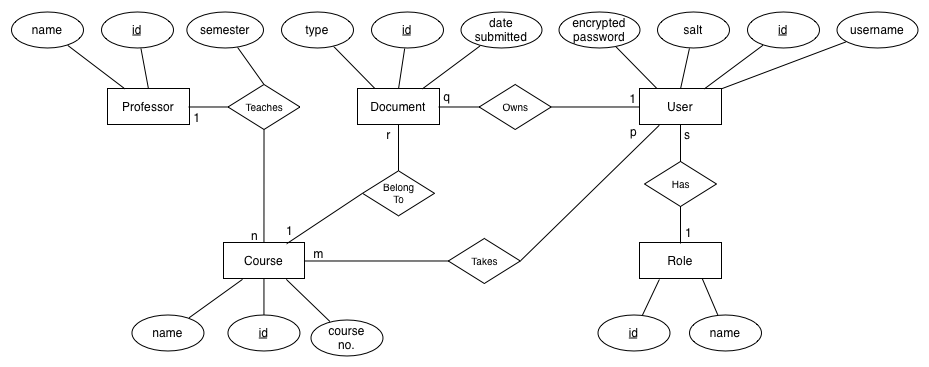
\includegraphics[width=.9\linewidth]{ER Diagram.png}

\end{document}